%%%%%%%%%%%%%%%%%%%%%%%%%%%%%%%%%%%%%%%%%
% Dreuw & Deselaer's Poster
% LaTeX Template
% Version 1.0 (11/04/13)
%
% Created by:
% Philippe Dreuw and Thomas Deselaers
% http://www-i6.informatik.rwth-aachen.de/~dreuw/latexbeamerposter.php
%
% This template has been downloaded from:
% http://www.LaTeXTemplates.com
%
% License:
% CC BY-NC-SA 3.0 (http://creativecommons.org/licenses/by-nc-sa/3.0/)
%
%%%%%%%%%%%%%%%%%%%%%%%%%%%%%%%%%%%%%%%%%

%----------------------------------------------------------------------------------------
%	PACKAGES AND OTHER DOCUMENT CONFIGURATIONS
%----------------------------------------------------------------------------------------

\documentclass[final,hyperref={pdfpagelabels=false}]{beamer}

\usepackage[orientation=portrait,size=a1,scale=1.3]{beamerposter} % Use the beamerposter package for laying out the poster with a portrait orientation and an a0 paper size

\usetheme{I6pd2} % Use the I6pd2 theme supplied with this template

\usepackage[english]{babel} % English language/hyphenation

\usepackage{amsmath,amsthm,amssymb,latexsym} % For including math equations, theorems, symbols, etc

%\usepackage{times}\usefonttheme{professionalfonts}  % Uncomment to use Times as the main font
%\usefonttheme[onlymath]{serif} % Uncomment to use a Serif font within math environments

\boldmath % Use bold for everything within the math environment

\usepackage{booktabs} % Top and bottom rules for tables

\graphicspath{{figures/}} % Location of the graphics files
\usepackage{graphicx}
\usepackage{wrapfig}
%\usepackage{floatrow}

\usecaptiontemplate{\small\structure{\insertcaptionname~\insertcaptionnumber: }\insertcaption} % A fix for figure numbering

%----------------------------------------------------------------------------------------
%	TITLE SECTION 
%----------------------------------------------------------------------------------------

\title{\huge A Sphere Model for Atrial Fibrillation} % Poster title

\author{Tigany Zarrouk \& Mattia Gaggi } % Author(s)

\institute{Supervisor: Kim Christensen.  Condensed Matter Theory Group---Imperial College London} % Institution(s)

%----------------------------------------------------------------------------------------
%	FOOTER TEXT
%----------------------------------------------------------------------------------------

\newcommand{\leftfoot}{} % Left footer text

\newcommand{\rightfoot}{} % Right footer text


%----------------------------------------------------------------------------------------

\begin{document}

\addtobeamertemplate{block end}{}{\vspace*{2ex}} % White space under blocks

\begin{frame}[t] % The whole poster is enclosed in one beamer frame

\begin{columns}[t] % The whole poster consists of two major columns, each of which can be subdivided further with another \begin{columns} block - the [t] argument aligns each column's content to the top

\begin{column}{.02\textwidth}\end{column} % Empty spacer column

\begin{column}{.465\textwidth} % The first column

%----------------------------------------------------------------------------------------
%	OBJECTIVES
%----------------------------------------------------------------------------------------



%----------------------------------------------------------------------------------------
%	INTRODUCTION
%----------------------------------------------------------------------------------------
            
\begin{block}{Introduction}


\textbf{Atrial Fibrillation} (AF) is a type of cardiac arrhythmia and one of the major causes of stroke and heart failure. AF is also the most widespread cardiac condition, with over 30 million people suffering from it worldwide. In the UK, expenses related to this disease account for more than 1 percent of the total National Health Service budget, costing more than 800 million pounds.\\*
 Atrial fibrillation usually manifests itself in patients with tachycardia, an abnormal hastening of cardiac beating.\\



\end{block}


\begin{block}{Phenomenology of the Heart}

\begin{columns}
\begin{column}{.54\textwidth}
	\begin{itemize}
	\item \textbf{\textit{Heartbeat Propagation}}: Each heartbeat originates as an electric signal in the sinoatrial (SA) node that propagates first into the atria, then through the atrioventricular (AV) node, through Purkinje fibres, into the lower reaches of the heart (Figure \ref{fig:heart}). The electric signal is conducted through the cardiac muscle cells due to polarisation (a change in voltage of the cell membrane) which contracts the cell \cite{Comtois}. 
	\end{itemize}
\end{column}

\begin{column}{.43\textwidth}
	%\begin{wrapfigure}[10]{R}{0.3\textwidth}
	\begin{figure}
	
	
	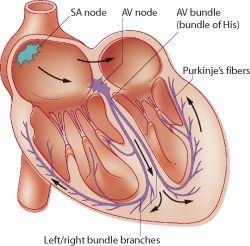
\includegraphics[width=0.85\textwidth]{heart}
	\caption{\label{fig:heart}This is the structure of the heart.}
	%\end{wrapfigure}
	\end{figure}
\end{column}
\end{columns}
\begin{itemize}

	\item \textbf{ \textit{Cells Excitation Rules}}: As the electric impulse propagates, each cardiac muscle cell can be in one of three stages:

		\begin{itemize}
 		 \item \textit{Rest/Excitable state}: the muscle cell is at rest with constant negative potential.								
  		\item \textit{Excited state}: the muscle cell is excited by adjacent excited cells it is connected to, making the voltage is at a maximum. 
  		\item \textit{Refractory state}: the muscle cell goes through a phase during which it can't be excited again---a steady decrease in voltage until its matches the rest state voltage---this period is called \textit{refractory period}. The refractory period duration is modulated by the cell excitation rate; this relationship is called \textit{restitution}.
		\end{itemize}  

\end{itemize}

\begin{columns}
\begin{column}{.43\textwidth}
\begin{figure}
	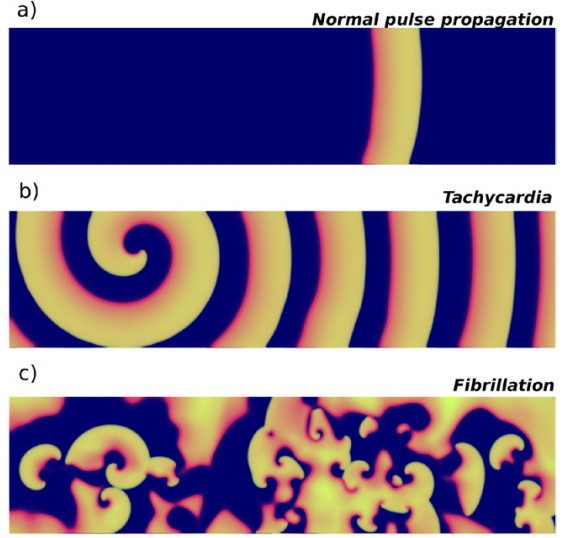
\includegraphics[width=0.95\textwidth]{spiralbreak2tachy}
	\caption{\label{fig:fib}Idealised diagram of: (a), normal heartbeat propagation; (b), tachycardia and (c), fibrillation. }
	%\end{wrapfigure}
	\end{figure}


\end{column}
\begin{column}{.54\textwidth}
\begin{itemize}
	\item \textbf{\textit{How AF Occurs}}: AF is correlated to the amount of \textbf{ fibrosis}---the scarring of cells. This creates dysfunctional/inactive cells, decreasing the number of connections between cells in the cardiac tissue. This promotes a process called \textit{reentry}, during which, the electric signal wavefront propagation chaotically breaks, initiating fibrillation \cite{Alonso}. Even though many treatments have been developed, the reentry mechanism is not completely understood and, as such, AF remains a major topic in medical research. \\
	\end{itemize}

	
	
\end{column}

\end{columns}

	\begin{itemize}
	
	
	%The current research revolves around three possible approaches:
 \item \textbf{\textit{Base for our Research}}: Our research is based on the work done by Christensen \emph{et al.}, which models the left atrium of the heart on a 2D surface \cite{Christensen}.
	\end{itemize}
\end{block}
\begin{block}{Our Objectives}

\begin{enumerate}
\item Replicate the model of the 2D cardiac atrium from Christensen \emph{et al.}
\item  Translate the model onto a sphere in order to simulate the effects of a more realistic morphology. 
\item Incorporate restitution of heart cells into the original model (such that the \textit{refractory period} of cells is modulated).
\item Observe the risk of AF in the new models and compare with the original model.
\end{enumerate}


\end{block}


\begin{block}{Sphere Model Morphology}

%\centering
\begin{figure}

\begin{columns}
\begin{column}{.67\textwidth}
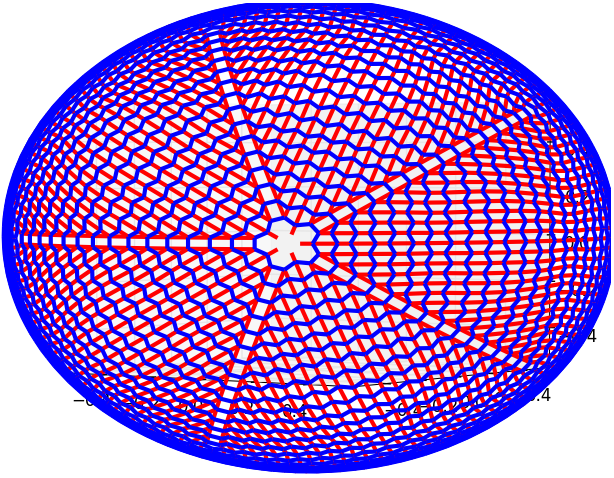
\includegraphics[width=0.8\linewidth]{connectome}

\end{column}
\hspace{-6em}
\begin{column}{.3\textwidth}
\caption{The structure of the sphere model. The connections in red (muscle fibres) are differentiated from the connection in blue (connections between fibres) in order to introduce fibrosis to the model. The effect of fibrosis is modelled by removing a percentage of the blue connections. Fibre growth from the SA node is seen.}

\end{column}
\end{columns}
\end{figure}

\end{block}


%\end{column}

%----------------------------------------------------------------------------------------

\end{column} % End of the first column

\begin{column}{.03\textwidth}\end{column} % Empty spacer column
 
\begin{column}{.465\textwidth} % The second column

%----------------------------------------------------------------------------------------
%	RESULTS
%----------------------------------------------------------------------------------------

%------------------------------------------------







\begin{block}{Implementing The Sphere Model}




In research by Fedotov, a model of the atrium was constructed on the surface of a triangulated sphere to model AF on a closed, heterogeneous surface \cite{Fedotov}. Inspired by this, we built a new model which translates Christensen \emph{et al.}'s model of a two dimensional atrium onto a sphere.


%\end{block}
%------------------------------------------------
%\begin{block}{Results: Sphere and Previous model}

%\centering
\begin{figure}
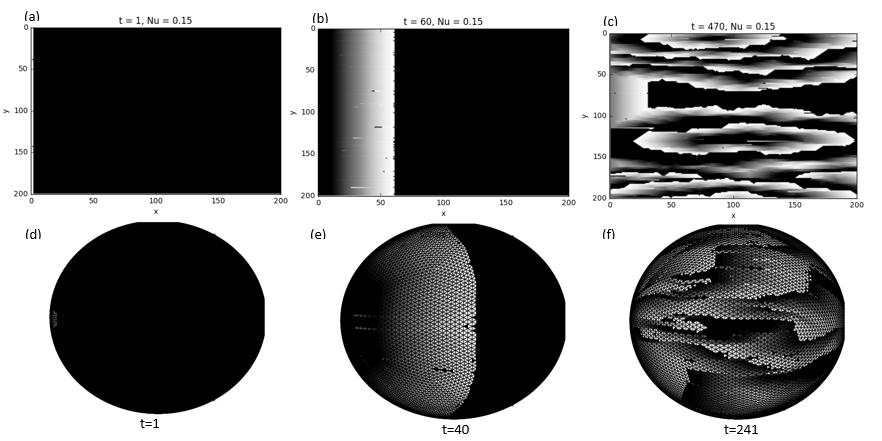
\includegraphics[width=0.8\linewidth]{combchristensenspherefib}
\caption{A comparison between Christensen \emph{et al.}'s model  (a, b and c)  and the sphere model (for d, e and f ) evolving in time in a fibrotic atrium. Normal wavefront propagation is seen starting in the leftmost figures .In figures b,e the excitation wavefront propagates unevenly due to fibrosis, initiating reentry. On the right, AF has spontaneously arisen from both models.}
\end{figure}

\end{block}

\begin{block}{Implementing the Restitution Model}

In Christensen \emph{et al.}'s model, the refractory period of each muscle cell was fixed.
In a real heart, the refractory period depends on the heart cell activation rate. The relationship between refractory period and cell excitation rate is called restitution. We introduced a linear restitution function into our replica of Christensen \emph{et al.}'s model in order to study its effects.
\end{block}


\begin{block}{Results: Risk of AF for the three models}

%\centering
\begin{figure}
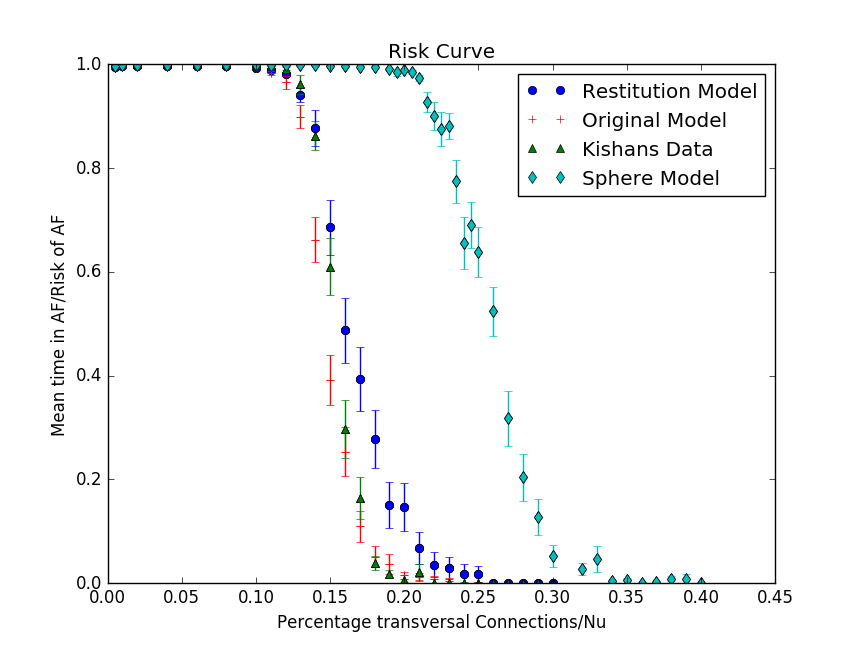
\includegraphics[width=0.65\linewidth]{xriskcurvesphere}
\caption{Risk of AF (defined as the fraction of time spent in fibrillation) for the three models studied: Christensen \emph{et al.}'s model ("Kishan's Data"); our original model; a restitution model and the sphere model. Each point is an average risk over 50 simulations, using a specified percentage of transversal connections ($\nu$), mimicking fibrosis levels. A healthy heart is expected to have $\nu$ close to 1 while a fibrotic heart has low $\nu$. Incorporating restitution into original model increases the risk. The sphere model incorporating fibre growth increases the risk further, producing a more realistic model as less fibrosis is necessary to induce AF. }
\end{figure}

\end{block}

%----------------------------------------------------------------------------------------
%	CONCLUSION
%----------------------------------------------------------------------------------------

\begin{block}{Conclusion}

A simplified mechanism of AF had been achieved by replication of Christensen \emph{et al.'s} model: simulating a sheet of atrial muscle tissue and incorporating the effects of fibrosis. We incorporated more features into this model: a more realistic heart morphology,with muscle fibre growth, using a sphere, and restitution. Our results show a higher risk of AF for the new models created. This produced more realistic models as less fibrosis is necessary to induce AF.
\end{block}

%----------------------------------------------------------------------------------------
%	REFERENCES
%----------------------------------------------------------------------------------------

\begin{block}{References}
\begin{thebibliography}{1}

%\nocite{*} % Insert publications even if they are not cited in the poster
%\small{\bibliographystyle{unsrt}
%\bibliography{sample1}}
\small
\bibitem{Comtois}
P. Comtois, J. Kneller, S. Nattel,
\emph{Of circles and spirals: Bridging the gap between the leading circle and spiral wave concepts of cardiac reentry}
Europace. 2005 Sep;7 Suppl 2:10-20.
DOI: http://dx.doi.org/10.1016/j.eupc.2005.05.011



\bibitem{Alonso}
S. Alonso, M. Bar and B. Echebarria
\emph{Nonlinear physics of electrical wave
propagation in the heart: a review},
Rep. Prog. Phys. 79 (2016) 096601, 
doi:10.1088/0034-4885/79/9/096601

\bibitem{Christensen}
Kim Christensen, Kishan A. Manani, and Nicholas S. Peters
\emph{Simple Model for Identifying Critical Regions in Atrial Fibrillation}
Phys. Rev. Lett. 114, 028104 – Published 16 January 2015



\bibitem{Fedotov}
N. M. Fedotov,  A. I. Oferkin, and S. V. Zhary,
\emph{Modeling Sources of Atrial Fibrillation on a Triangulated Sphere}
Biomedical Engineering, Vol. 49, No. 2, July, 2015, pp. 112115. 
\end{thebibliography}

\end{block}



%----------------------------------------------------------------------------------------
%	CONTACT INFORMATION
%----------------------------------------------------------------------------------------

%\setbeamercolor{block title}{fg=black,bg=orange!70} % Change the block title color

%\begin{block}{Contact Information}

%\begin{itemize}
%\item Web: \href{http://www.university.edu/smithlab}{http://www.university.edu/smithlab}
%\item Email: \href{mailto:john@smith.com}{john@smith.com}
%\item Phone: +1 (000) 111 1111
%\end{itemize}

%\end{block}

%----------------------------------------------------------------------------------------

\end{column} % End of the second column

\begin{column}{.015\textwidth}\end{column} % Empty spacer column

\end{columns} % End of all the columns in the poster

\end{frame} % End of the enclosing frame

\end{document}